%Made By Thomas Debelle
\documentclass{report}
\usepackage[a4paper, total={6in, 9in}]{geometry}
\usepackage[utf8]{inputenc}
\usepackage[francais]{babel}
\usepackage{graphicx}
\usepackage{graphics}
\usepackage[T1]{fontenc}
\usepackage{amsmath}
\usepackage{hyperref}
\usepackage{amssymb}
\usepackage{listings}
\usepackage{xcolor}
\usepackage{array}
\usepackage{float}
\usepackage{amsfonts}
\usepackage{fancyhdr}
\usepackage{titlesec}
\usepackage{xparse}
\usepackage{wrapfig}

\hypersetup{
    colorlinks=true,
    linkcolor=black,
    filecolor=magenta,
    urlcolor=cyan,
    pdftitle={Overleaf Example},
    pdfpagemode=FullScreen,
    }
\begin{document}


\begin{titlepage}
    \begin{figure}
        
\includegraphics[height = 2cm]{UCL_Logo.png}
        \label{fig:my_label}
    \end{figure}

    \hspace*{100cm}
    \centering
    \vspace*{7cm}

    {\Huge \textbf{Résumé de LEPL1106}}\\
    \vspace*{0.25cm}
    compilation du \today\\
    \vspace*{0.25cm}
    \Large{Thomas Debelle}\\

    \vspace*{9.5cm}
    {\Large Juin 2023}
\end{titlepage}


\tableofcontents
\newpage

\section*{Préface}

Bonjour à toi !\\

Cette synthèse recueille toutes les informations importantes données au cours, pendant les séances de tp et est amélioré grâce au note du Syllabus. Elle ne remplace pas le cours donc écoutez bien les conseils et potentielles astuces que les professeurs peuvent vous donner. Notre synthèse est plus une aide qui on l'espère vous sera à toutes et tous utiles.\\

Elle a été réalisée par toutes les personnes que tu vois mentionné. Si jamais cette synthèse a une faute, manque de précision, typo ou n'est pas à jour par rapport à la matière actuelle ou bien que tu veux simplement contribuer en y apportant ta connaissance ? Rien de plus simple ! Améliore la en te rendant \href{http://www.github.com/Tfloow/Q4_EPL}{ici} où tu trouveras toutes les infos pour mettre ce document à jour. (\textit{en plus tu auras ton nom en gros ici et sur la page du github})\\

Nous espérons que cette synthèse te sera utile d'une quelconque manière ! Bonne lecture et bonne étude.


\part{Signaux}

\chapter{Les signaux}
\section{Définition}
\subsubsection{Définition}
Un signal est une fonction de une ou plusieurs variables (continues ou discrètes) qui correspondent à de l'information ou a un phénomène physique.

\subsubsection{Continues ou discrets ?}
Un signal est dit continu si il est définit sur un espace de temps continu. On note ce signal $x(t)$. Et il est dit discret si il est définit sur un espace discret de temps. On note ce signal $x[t]$.

\subsubsection{Manipulation des signaux}
Pour le cas discrets ou continu, nous pouvons réaliser les opérations suivantes.
\begin{itemize}
\item Combinaison linéaire $\rightarrow \alpha_{1}x_{1}(t) + \alpha_{2}x_{2}(t)$
\item Multiplication $ \rightarrow x_{1}[t]x_{2}[t]$
\item Dilatation $ \rightarrow x[n/a], a > \mathbb{R}$
\item Translation $ \rightarrow x(t - t_0), t_0 \in \mathbb{R}$
\item Renversement $ \rightarrow x(-t)$
\item Différentiation (que pour le cas continu) $ \rightarrow \frac{d^n x(t)}{dt^n}$
\item Intégration (que pour le cas continu)
\end{itemize}

\section{Signaux élémentaires}
\subsection{Signaux exponentiels}
Pour les signaux continus nous avons:
\begin{equation}
x(t) = B e^{at}
\end{equation}
Et pour les signaux discrets nous avons:
\begin{equation}
x[n] = Br^n \rightarrow 0 < r < 1
\end{equation}

\subsection{Signaux sinusoïdales}
Pour les signaux continus nous avons:
\begin{equation}
x(t) = A cos(\omega t + \phi)
\end{equation}
Et pour les signaux discrets nous avons:
\begin{equation}
x[n] = A cos(\Omega n + \Phi)
\end{equation}
Il a une période de $\Omega N = 2 \pi m$

\subsection{Signaux amortis}
Pour les signaux continus et avec $\alpha > 0$:
\begin{equation}
x(t) = A e^{-\alpha t}cos(\omega t + \phi)
\end{equation}
Et pour les signaux discrets:
\begin{equation}
x[n] = Br^ncos(\Omega n + \Phi)
\end{equation}

\subsection{L'impulsion (temps discret)}
Comme son nom l'indique, ce signal se représente sous la forme d'une impulsion. Par sa définition, cela nous force a avoir un signal discret !
\begin{equation}
\begin{cases}
\delta [n] = 1 \rightarrow n = 0 \\
\delta [n] = 0 \rightarrow \forall n \notin 0
\end{cases}
\end{equation}
On peut réaliser des impulsions décaler en écrivant $\delta [n-x]$ avec $x$ représentant la valeur du décalage.

\subsection{L'échelon (temps discret)}
Ce type de signal élémentaire est encore plus trivial puisqu'il se résume à:
\begin{equation}\label{eq:1}
\begin{cases}
1 \rightarrow n \geq 0 \\
0 \rightarrow n < 0
\end{cases}
\end{equation}
On peut aussi voir l'échelon comme une somme infinie d'impulsion comme $\sum_{k \geq 0}^{\infty} \delta[n-k]$.\\
Il existe également un échelon en temps continu qui se résume à la même équation \ref{eq:1} mais pour des valeurs continues.

\subsection{L'impulsion (temps continu)}
\begin{equation}
\begin{cases}
\delta (t) = 0 si t \neq 0\\
\delta (0) = ?(+\infty)\\
\int_{-a}^a \delta (s) ds = 1 \rightarrow \forall a > 0
\end{cases}
\end{equation}
A noter que la dernière ligne nous crée une propriété bien spécifique. En effet, la valeur de l'impulsion est limité par les bornes $a$ puisqu'on impose une intégrale égale à 1.

\subsubsection{Lien entre impulsion et échelon}
$\delta (t) = u'(t)$ donc l'impulsion est une sorte de dérivé de l'échelon.

\section{Convolution}
La convolution est une nouvel opérateur qui nous sera très utile. Son signe est "$\ast$" et la formule qui définit cette opération est:
\begin{equation}
f[n] \ast g[n] := \sum_{k=-\infty}^{\infty} f[k]g[n-k] 
\end{equation}
La méthode pour trouver le résultat d'une convolution est:
\begin{enumerate}
\item Il faut "\textit{renverser}" une des fonctions. C'est-à-dire faire $f[n] \rightarrow f[-n]$.
\item Puis multiplier ces deux nouvelles fonctions.
\item L'\textit{aire} sous la courbe créer par cela est le résultat de la convolution.
\end{enumerate}

\section{Modélisation et représentation des systèmes}
Comme vu précédemment, la réponse impulsionelle est le résultat du système étant perturbé par une impulsion. 
\subsection{Inconvénient}
\begin{enumerate}
\item Fonction de taille \textit{infinie} et représentation donc \textit{peu simple}.
\item La modélisation d'un système ne mène généralement pas à une réponse impulsionelle .
\item On doit connaitre l'entrée depuis $-\infty$
\end{enumerate}

\subsection{Représentation}
\begin{wrapfigure}{r}{.3\textwidth}
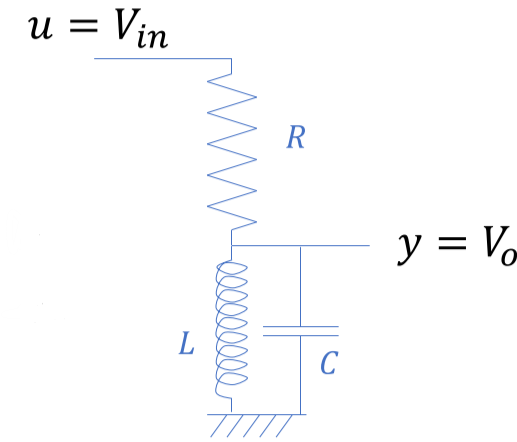
\includegraphics[width=5cm]{img/RLC.png}
\caption{Circuit RLC}
\label{fig:RLC}
\end{wrapfigure}
Il existe 3 grandes façons de représenter un système. Tout d'abord la méthode \textit{équation différentielle d'entrée-sortie}. Pour la suite des exemples, j'utiliserai un circuit \textit{RLC} comme montré ci-contre.\\

\textit{équation différentielle d'entrée-sortie} est une somme des dérivées comme montré dans l'équation \ref{eqn:es}. C'est plutôt facile de trouver les équations mais on fait face à un problème, l'opération \textit{dérivée} n'existe pas dans le monde réelle, il faut un opérateur intégrateur.\\

Ensuite, nous avons la \textit{représentation d'état} qui utilise des matrices pour former les équations différentielles comme nous voyons à l'équation \ref{eqn:mat}\\

La dernière représentation type est le \textit{schéma bloc} qui est visuel et qui utilise lui des blocs intégrateurs au lieu de dérivé comme montré à la figure \ref{fig:bloc}.

\begin{equation} \label{eqn:es}
\ddot{y} + \frac{1}{CR}\dot{y} + \frac{1}{LC}y = \frac{1}{CR}\dot{u}
\end{equation}

\begin{equation} \label{eqn:mat}
\frac{d}{dt}\begin{pmatrix}
V_0\\
I_L
\end{pmatrix} = \begin{pmatrix}
-1/RC & -1/C\\
1/L & 0
\end{pmatrix} \begin{pmatrix}
V_0\\
L
\end{pmatrix} + \begin{pmatrix}
1/RC\\
0
\end{pmatrix} u
\end{equation}

\begin{figure}[H] 
\centering
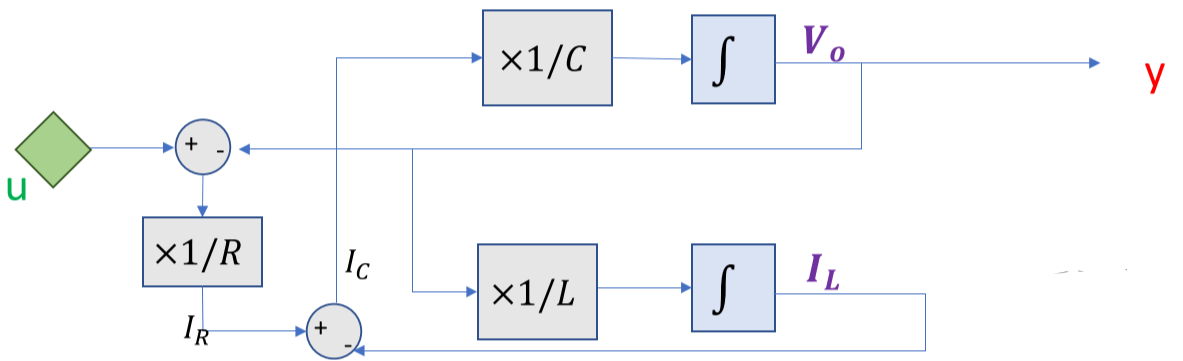
\includegraphics[width=7cm]{img/bloc.png}
\caption{Repésentation \textit{bloc} du système à la figure \ref{fig:RLC}}
\label{fig:bloc}
\end{figure}

\subsection{Équation différentielle entrée-sortie}
La forme générale de ces équations est de ce type:
\begin{equation}\label{eqn:difes}
\sum_{k = 0}^{N} a_k (\frac{d^k}{dt^k}) y(t) = \sum_{k = 0}^M b_k (\frac{d^k}{dt^k}) u(t)
\end{equation}
Quelque chose à bien remarquer est que ces équations ne modélise \textit{qu'une partie} d'un système \textit{LIT}. Par exemple, on ne peut pas représenter un \textit{délai} ce qui également rare dans la réalité.\\

Une chose à remarquer est que l'opérateur \textit{dérivé} peut se "\textit{démultiplier}" et possède une \textit{associativité} et \textit{commutativité}. Ainsi, on peut avoir une représentation dite "\textit{polynomiale}" comme ci-dessus qui est une autre écriture de l'équation \ref{eqn:difes}.
\begin{equation}\label{eqn:poly}
p(\frac{d}{dt})y(t) = q (\frac{d}{dt})u(t)
\end{equation}
Puis après, pour résoudre ce genre d'équation, on utilise des méthodes classiques vu au cours d'Analyse donc, solution homogène et particulière ...

\subsubsection{Réponse libre et forcée}
Une réponse \textit{libre} est la solution de l'équation homogène, donc quand $u(t) = 0$ à l'équation \ref{eqn:poly} et on garde les \textbf{mêmes conditions initiales}. En somme c'est la représentation de l'impact des \textit{CI}.\\

Une réponse \textit{forcée} est l'équation \ref{eqn:poly} mais avec les \textit{conditions initiales} nulles. Donc on s'intéresse à l'impact de l'entrée sans les conditions initiales. La somme de la réponse \textit{libre} et \textit{forcée} nous donne la réponse générale.

\subsubsection{Stabilité}
On peut avoir une intuition sur la stabilité de notre système en posant $y_H(t)$ qui équivaut à:
\begin{equation}
y_H(t) = \sum_i \alpha_ie^{r_it} \rightarrow \quad r_i \text{ correspond aux racines de p(z) de \ref{eqn:poly}}
\end{equation}
Si la partie réelle de $r_i < 0 \forall i$ alors on a une exponentielle décroissante donc \textbf{stable}. On appelle ce genre de système \textit{BIBO} stable ou \textit{Bounded Input Bounded Output}.\\

En revanche, si $r_i > 0 \exists i$ donc on a au moins une exponentielle croissante créant une \textit{instabilité}.\\

Si $r_i = 0 \exists i$ on dit qu'on a une \textit{stabilité marginale} ou \textit{instabilité}. Cela dépendera de la \textbf{multiplicité} et de \textbf{$te^{r_it}$}.

\subsubsection{Linéarité de l'entrée}
Avec cette représentation polynomiale, on peut facilement voir qu'on a une linéarité de l'entrée nous permettant de simplifier différent calcul. %rajouter la formule etc

\subsubsection{Avantages et Inconvénients}
2 représentations qui sont \ref{eqn:difes} et \ref{eqn:poly}. Les avantages:
\begin{itemize}
\item Représentation compacte.
\item Conditions initiales claires.
\item Facile de la transformer dans d'autres représentations.
\end{itemize}
Les désavantages:
\begin{itemize}
\item On peut perdre la représentation physique.
\end{itemize}

\subsection{Schéma Bloc}
Comme son nom l'indique, le schéma bloc utilise des "\textit{blocs}" pour représenter notre système. Ci-dessus on peut voir les composants de base composant ce type de schéma
\begin{figure}[H]
\centering
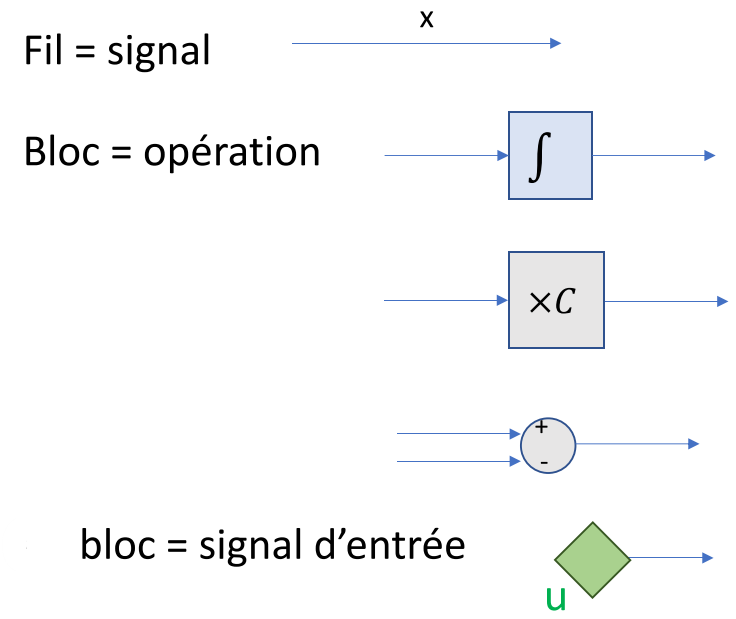
\includegraphics[width=5cm]{img/blocExemple.png}
\caption{Liste reprenant les blocs de base}
\end{figure}
Dans le cadre des systèmes \textit{LIT}, on se restreint souvent à l'addition, multiplication et intégration. On ne réalise que des opérations \textit{linéaires}.

\subsubsection{Avantages et Inconvénients}
Les avantages:
\begin{itemize}
	\item Représentation très intuitive.
	\item Proche de l'implémentation réelle du système.
	\item On peut plus facilement réfléchir sur le \textit{design} de notre système.
	\item Très modulaire.
\end{itemize}
Les désavantages:
\begin{itemize}
	\item Lien moins clair avec la solution.
\end{itemize}
De plus, on peut voir comme un \textit{avantage} ou \textit{inconvénient} le fait de pouvoir voir l'évolution des signaux entre chaque bloc plutôt qu'une sorte de boite noire "\textit{entrée-sortie}". De plus, on peut réaliser de bien des manières des circuits.

\subsection{Représentation d'état}
Dans ce type de représenation, on a \textcolor{red}{état $x$} qui est un \textit{vecteur} comportant toutes les infos internes de notre système. On \textcolor{red}{entrée $u$} qui est un \textit{signal} extérieur affectant le système. Finalement on a une \textcolor{red}{sortie $y$} qui est un signal qu'on peut accéder depuis l'extérieur.\\
\begin{equation}
\begin{cases}
\text{évolution: }\frac{d}{dt}x(t) =  Ax(t) + Bu(t)\\
\text{sortie: } C x(t) + D u(t)
\end{cases}
\end{equation}

\subsubsection{Solution}
La solution \textit{homogène} de $e^{\lambda_it}$ avec $\lambda_i$ étant les valeurs propres de l'équation. Si la partie réelle des racines est négative pour tout $\lambda_i$.

\subsubsection{État non-unique}
Avec cette représentation, on peut facilement modifier les vecteurs et signaux pour rendre les équations plus simples. Cela n'a aucun impacte et rend les équations plus logiques pour un certain sens "\textit{réel}".
\begin{equation}
\begin{cases}
z = Tx \Rightarrow \frac{d}{dt}z = T\frac{d}{dt}x = TAT^{-1}z(t) + TBu(t)\\
y = Cx(t) + Bu(t) = CT^{-1}z(t) + Du(t) 
\end{cases}
\end{equation}

Si la matrice $A$ est diagonalisable, on peut réaliser un \textbf{découplage} et obtenir ainsi un mode dit \textit{découplé}. On peut également faire des \textit{blocs de Jordan} pour diagonaliser le tout:
\begin{equation}
\frac{d}{dt} z_i = \lambda_i z_i + \tilde{B}_i u
\end{equation}

\subsection{Passage de représentation}


\part{Systèmes}



\end{document}
